% Drawing 154/02-12 -- folder 154, batch 02, archive page 37 (PDF page 38).
% Transcription: figures : trois disques au bord vert, traversés de cordes orange, reliés par des flèches $\mapsto$ et $\leftarrow$ ; sur le premier, deux cordes $D$, $D'$ se rejoignent en haut et en bas en deux petits segments verts ; le deuxième est couvert de hachures au crayon ; sur le troisième les extrémités de $D$ et $D'$ sont écartées en haut, croisées en bas ($D'$, $D$), un petit triangle orange au bas du bord
% Kind: three chord systems in disks, joined by arrows. Method 2 (schematic redraw from the facsimile). Status: partial.
% Notes: Three disks with green rims crossed by orange chords, joined by the arrows |-> and <-: on the first, two chords D, D' meet at the top and at the bottom in two short green segments; the second is covered with pencil hatching; on the third the ends of D and D' are apart at the top and crossed at the bottom (D', D), a small orange triangle at the bottom of the rim. Read from the page view; the chords are schematic. The small figure lower in the column (a cross on a line with |-> and <-, and a disk at the foot of the page) is not covered by the marks of this page. Still differs from the facsimile: Read from the page view; the chords are schematic. The small figure lower in the column (a cross on a line with |-> and <-, and a disk at the foot of the page) is not covered by the marks of this page. 2 coloured or hatched triangle(s) are placed schematically and are not bounded by the strands that bound them on the page (1 now attached exactly).
% Coordinates: 1 unit = 1 mm = 1/100 of the crop width (bbox in page fractions: [0.56, 0.134, 0.859, 0.217]).
% Redrawn by Claude (claude-opus-5-5), issue #73, 2026-11-07; not checked by a human; not compiled (no TeX in the session).
% Revised by Claude (claude-opus-5-5) 2026-11-09 (issue #128) after Michel's check: vertices snapped to exact intersections (drawn points on their lines, meeting ends on the stroke they meet, near-concurrent lines through one computed point, curve ends on their rim); labels at \small as in folder 80 batch 3. Status: partial.
% Rights: reproduces part of the work -- behind RENDER_TRANSCRIPTS, never published by itself.
\documentclass[tikz,border=3pt]{standalone}
\usepackage{amsmath,amssymb}
\usetikzlibrary{patterns,arrows.meta}
\tikzset{Or/.style={orange!90!black}, Ye/.style={yellow!80!orange}, Lg/.style={green!60!black!70}, Dg/.style={green!45!black}, Br/.style={brown!80!black}, Rd/.style={red!85!black}, Bl/.style={blue!70!black}, Gy/.style={black!40}, pencil/.style={black!45}, struck/.style={black!35}, mark/.style={circle,draw,inner sep=1.3pt}, pt/.style={circle,fill,inner sep=0.9pt}, opt/.style={circle,draw,fill=white,inner sep=1.1pt}}
\begin{document}
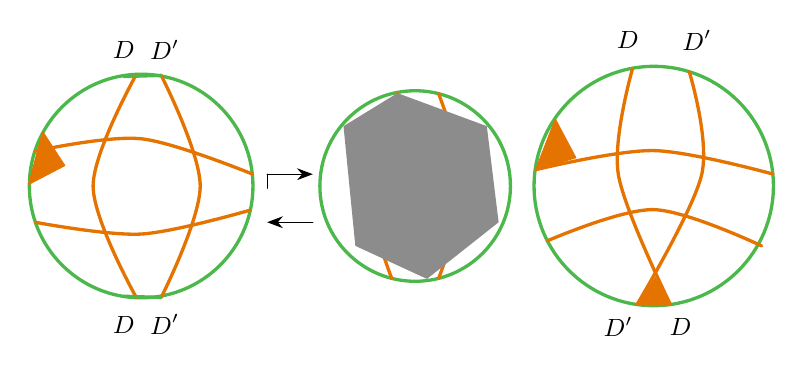
\begin{tikzpicture}[x=1mm,y=1mm,line cap=round,line join=round,font=\scriptsize]
\draw[Lg,very thick] (16.7,-21.2) circle[radius=14.2];
\draw[Or,very thick] plot[smooth, tension=0.55] coordinates {(16.1,-7.01) (10.6,-21.2) (16.1,-35.39)};
\draw[Or,very thick] plot[smooth, tension=0.55] coordinates {(19.25,-7.15) (24.2,-21.2) (19.25,-35.35)};
\draw[Lg,very thick] (14.5,-7.3) -- (19.25,-7.15);
\draw[Lg,very thick] (14.5,-35.2) -- (19.25,-35.35);
\draw[Or,very thick] plot[smooth, tension=0.55] coordinates {(3.21,-16.77) (16.7,-15.2) (30.82,-19.68)};
\draw[Or,very thick] plot[smooth, tension=0.55] coordinates {(3.27,-25.81) (16.7,-27.3) (30.57,-24.26)};
\draw[Or] (4.2,-14.3) -- (2.4,-21) -- (7,-18.6) -- cycle;
\fill[pattern=north east lines,Or] (4.2,-14.3) -- (2.4,-21) -- (7,-18.6) -- cycle;
\node[inner sep=1pt] at (14.5,-3.9) {\small $D$};
\node[inner sep=1pt] at (19.7,-3.9) {\small $D'$};
\node[inner sep=1pt] at (14.5,-38.8) {\small $D$};
\node[inner sep=1pt] at (19.7,-38.8) {\small $D'$};
\draw[-{Stealth[length=2mm]}] (32.7,-19.7) -- (38.5,-19.7);
\draw (32.7,-19.7) -- (32.7,-21.5);
\draw[-{Stealth[length=2mm]}] (38.5,-25.8) -- (32.7,-25.8);
\draw[Lg,very thick] (51.5,-21.2) circle[radius=12.1];
\draw[Or,very thick] plot[smooth, tension=0.55] coordinates {(49.25,-9.4) (45.5,-21.2) (48.52,-32.93)};
\draw[Or,very thick] plot[smooth, tension=0.55] coordinates {(54.48,-9.47) (57.6,-21.2) (54.48,-32.93)};
\fill[pattern=north east lines,pencil] (42.4,-13.6) -- (49.25,-9.4) -- (60.6,-13.6) -- (62.1,-25.8) -- (53,-33) -- (43.9,-28.8) -- cycle;
\draw[Lg,very thick] (81.8,-21.2) circle[radius=15.2];
\draw[Or,very thick] plot[smooth, tension=0.55] coordinates {(79.12,-6.24) (77.3,-19.7) (83.92,-36.25)};
\draw[Or,very thick] plot[smooth, tension=0.55] coordinates {(86.31,-6.68) (87.9,-19.7) (79.68,-36.25)};
\draw[Or,very thick] plot[smooth, tension=0.55] coordinates {(66.8,-19.13) (81.8,-16.7) (96.92,-19.68)};
\draw[Or,very thick] plot[smooth, tension=0.55] coordinates {(68.29,-28.16) (81.8,-24.2) (95.5,-28.8)};
\draw[Or] (69.3,-12.7) -- (66.8,-19.13) -- (71.9,-17.6) -- cycle;
\fill[pattern=north east lines,Or] (69.3,-12.7) -- (66.8,-19.13) -- (71.9,-17.6) -- cycle;
\draw[Or] (79.69,-36.24) -- (80.48,-36.34) -- (81.8,-36.4) -- (83.12,-36.34) -- (83.91,-36.24) -- (83.84,-36.13) -- (83.62,-35.77) -- (83.28,-35.19) -- (82.84,-34.41) -- (82.32,-33.46) -- (82,-32.84) -- (81.63,-33.43) -- (80.99,-34.39) -- (80.45,-35.18) -- (80.04,-35.76) -- (79.77,-36.13) -- cycle;
\fill[pattern=north east lines,Or] (79.69,-36.24) -- (80.48,-36.34) -- (81.8,-36.4) -- (83.12,-36.34) -- (83.91,-36.24) -- (83.84,-36.13) -- (83.62,-35.77) -- (83.28,-35.19) -- (82.84,-34.41) -- (82.32,-33.46) -- (82,-32.84) -- (81.63,-33.43) -- (80.99,-34.39) -- (80.45,-35.18) -- (80.04,-35.76) -- (79.77,-36.13) -- cycle;
\node[inner sep=1pt] at (78.5,-2.7) {\small $D$};
\node[inner sep=1pt] at (87.3,-2.7) {\small $D'$};
\node[inner sep=1pt] at (77.3,-39.1) {\small $D'$};
\node[inner sep=1pt] at (85.2,-39.1) {\small $D$};
\end{tikzpicture}
\end{document}
